\documentclass{article}

\usepackage[portuguese]{babel}

\usepackage{amsmath, amssymb}
\usepackage{graphicx}
\usepackage[colorlinks=true, allcolors=blue]{hyperref}

\usepackage[section]{placeins}

\title{Lista 04}
\author{Vinícius de Oliveira Peixoto Rodrigues (245294)}
\date{Setembro de 2022}

\begin{document}
\maketitle

\section*{Questão 1}

O código abaixo, que pode ser executado em uma SageCell (\url{https://sagecell.sagemath.org/}), implementa uma troca de chaves de Diffie-Hellman, mostrando que Ana e Beto chegam à mesma chave de sessão:

\begin{verbatim}
    p = 223870593518163443859383880946274616097; r = 5
    k_pr_a = 245294; k_pr_b = 492542;
    k_pu_a = (r ^ k_pr_a) % p; k_pu_b = (r ^ k_pr_b) % p;
    k_a = (k_pu_b ^ k_pr_a) % p; k_b = (k_pu_a ^ k_pr_b) % p;
    (k_a, k_b)

    Output:
    (81356090094332686708875839913537404335,
     81356090094332686708875839913537404335)
\end{verbatim}

\section*{Questão 2}

Algumas das vantagens do ECC sobre o RSA são:

\begin{itemize}
    \item Maior segurança: é muito mais difícil calcular o logaritmo de curva elíptica do que fatorar números usand o o General Number Sieve
    \item Como consequência do item acima, o ECC necessita de tamanhos de chave significativamente menores que o RSA (mais vantajoso em sistemas embarcados, com recursos limitados)
    \item O ECC é também significativamente mais rápido que o ECC devido aos tamanhos de chave menores
\end{itemize}

\section*{Questão 3}

Uma curva elíptica arbitrária

\begin{equation*}
    y^2 = x^3 + ax + b
\end{equation*}

deve satisfazer a condição de que o determinante $\Delta = -16 (4a^3 + 27b^2)$ deve ser não-nulo ou, equivalentemente, o polinômio $x^3 + ax + b$ deve ter raízes distintas; isso garante que a curva não será degenerada.

\section*{Questão 4}

Uma curva elíptica sobre os reais é um lugar geométrico (i.e. conjunto de soluções $\{(x,y)\}$) que atende à condição $y^2 = x^3 + ax + b$.

Um grupo elíptico módulo $p$, $E_p(a,b)$, é análogo a uma curva elíptica mas atua sobre um grupo finito cíclico $\mathbb{Z}_p$, com $p$ primo, de modo que é definido como o conjunto de soluções da equação $y^2 \equiv x^3 + ax + b \mod p$ (todas as soluções sendo elementos de $\mathbb{Z}_p$, i.e., inteiros módulo $p$). É possível ainda definir uma operação de soma $\oplus$ de modo que o conjunto das soluções de $y^2 \equiv x^3 + ax + b \mod p$, associado a essa operação, formam um grupo abeliano.

\section*{Questão 5}

A operação-chave do ECC é a seguinte: dada uma curva elíptica sobre um grupo finito, é possível definir uma operação de soma $\oplus$ de modo que o conjunto dos pontos da curva associados à operação de soma formam um grupo abeliano $G$.

Define-se em seguida, para um ponto $P \in G$ a operação 
\begin{equation*}
    kP = \underbrace{P \oplus P \oplus + ... \oplus P}_{k\text{ vezes}}
\end{equation*}

No ECC, usa-se um valor grande de $k$, normalmente com algumas centenas de bits. É possível calcular $kP$ relativamente rápido. Seja $k = b_0 b_1 ... b_{n}$ a representação binária de $k$; é possível calcular $R = kP$ em tempo logarítmico:

\begin{itemize}
    \item calculamos inicialmente os valores de $(2^i)P$, $i = {0,1,...,n}$
    \item calculamos $R = kP$ observando que $kP = (\sum_{i=0}^{n} b_i2^{i})P = \underbrace{\sum_{i=0}^{n}b_i(2^{i}P)}_{\log_2(n) \text{ operações}}$ (visto que $G$ é um grupo abeliano)
\end{itemize}

O problema inverso (conhecido como logaritmo de curvas elípticas), de calcular um $k$ tal que $kP = R$, é muito mais complicado e os melhores algoritmos conhecidos atualmente têm complexidade exponencial. Desse modo, a operação $kP$ funciona como uma função de mão única: é fácil calcular $kP$ em tempo logarítmico, mas o caminho inverso tem complexidade exponencial.

\section*{Questão 6}

O seguinte código gera todos os pontos em $E_p(a, b)$:

\begin{verbatim}
    E = EllipticCurve(GF(23), [1, 12])
    print(E.points())
    E.plot()

    Output:
    [(0 : 1 : 0), (0 : 9 : 1), (0 : 14 : 1), (5 : 2 : 1), (5 : 21 : 1),
    (6 : 2 : 1), (6 : 21 : 1), (8 : 7 : 1), (8 : 16 : 1), (12 : 2 : 1),
    (12 : 21 : 1), (19 : 6 : 1), (19 : 17 : 1), (21 : 5 : 1), (21 : 18 : 1)]
\end{verbatim}


\begin{figure}[!ht]
    \begin{center}
        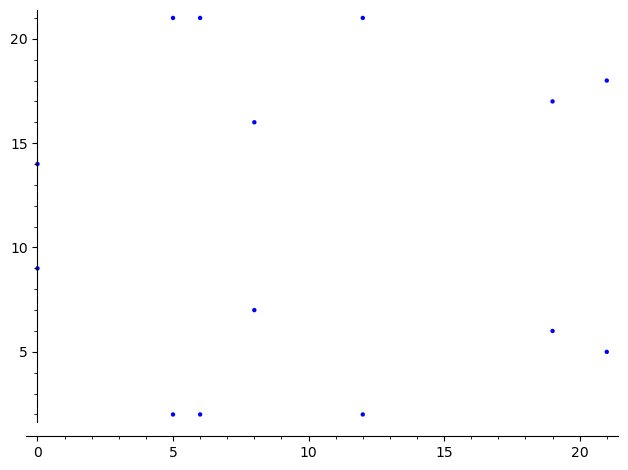
\includegraphics[width=\textwidth]{images/q6.png}
    \end{center}
\end{figure} 
\FloatBarrier

\section*{Questão 7}

\begin{verbatim}
    E = EllipticCurve(GF(23), [1, 12])
    xp = 21; yp = 5
    xq = 0; yq = 9
    L = (yp-yq)/(xp-xq)
    xr = (L^2 - xp - xq) % 23
    yr = (L*(xp - xr) - yp) % 23
    print(f"({xr}, {yr})")
    print(E(xp, yp) + E(xq, yq))
    
    Output:
    (6, 2)
    (6 : 2 : 1)
\end{verbatim}

\section*{Questão 8}

\begin{verbatim}
    # brainpoolP256r1 according to RFC5639
    p = 0xA9FB57DBA1EEA9BC3E660A909D838D726E3BF623D52620282013481D1F6E5377
    a = 0x7D5A0975FC2C3057EEF67530417AFFE7FB8055C126DC5C6CE94A4B44F330B5D9
    b = 0x26DC5C6CE94A4B44F330B5D9BBD77CBF958416295CF7E1CE6BCCDC18FF8C07B6
    x = 0x8BD2AEB9CB7E57CB2C4B482FFC81B7AFB9DE27E1E3BD23C23A4453BD9ACE3262
    y = 0x547EF835C3DAC4FD97F8461A14611DC9C27745132DED8E545C1D54C72F046997
    n = 0xA9FB57DBA1EEA9BC3E660A909D838D718C397AA3B561A6F7901E0E82974856A7

    # private keys (both in [0, n-1])
    d_a = 0x616c696365 # "alice" in ascii
    d_b = 0x626f626f62 # "bobob" in ascii

    E = EllipticCurve(GF(p), [a,b])
    G = E(x, y)

    # public keys
    Q_a = d_a * G
    Q_b = d_b * G

    key_a = d_a * Q_b
    key_b = d_b * Q_a

    print(key_a == key_b) # key has been shared

    Output:
    True
\end{verbatim}

\section*{Questão 9}

De acordo com \url{https://en.wikipedia.org/wiki/Elliptic_Curve_Digital_Signature_Algorithm}:

\begin{verbatim}
    import hashlib

    p = 0xA9FB57DBA1EEA9BC3E660A909D838D726E3BF623D52620282013481D1F6E5377
    a = 0x7D5A0975FC2C3057EEF67530417AFFE7FB8055C126DC5C6CE94A4B44F330B5D9
    b = 0x26DC5C6CE94A4B44F330B5D9BBD77CBF958416295CF7E1CE6BCCDC18FF8C07B6
    x = 0x8BD2AEB9CB7E57CB2C4B482FFC81B7AFB9DE27E1E3BD23C23A4453BD9ACE3262
    y = 0x547EF835C3DAC4FD97F8461A14611DC9C27745132DED8E545C1D54C72F046997
    n = 0xA9FB57DBA1EEA9BC3E660A909D838D718C397AA3B561A6F7901E0E82974856A7
    
    E = EllipticCurve(GF(p), [a,b])
    G = E(x, y)
    
    # private keys
    d_a = 0x616c696365 # "alice" in ascii
    
    # public keys
    Q_a = d_a * G
    
    # signature generation
    
    # "random" number for illustrative purposes
    k = 0xDEADBEEF
    
    text = b"""Lorem ipsum dolor sit amet, consectetur adipiscing elit.
    Praesent sit amet faucibus odio,
    non ornare ipsum. Phasellus id lacinia lectus.
    Sed vitae auctor sem. Praesent sollicitudin in lectus nec dapibus.
    Class aptent taciti sociosqu ad litora
    torquent per conubia nostra, per inceptos himenaeos."""
    
    z = int(hashlib.sha256(text).hexdigest(), 16) # has bit length of 256, same as n
    
    P = k*G
    x1 = P[0]
    _, k_inv, _ = xgcd(k, n)
    
    r = Integer(mod(x1, n))
    s = Integer(mod(k_inv*(z + r*d_a), n))
    
    # signature verification
    
    # after user receives text and calculates hash
    _, s_inv, _ = xgcd(s, n)
    u1 = mod(z*s_inv, n); u2 = mod(r*s_inv, n)
    P = u1*G + u2*Q_a
    P[0] == r # verification

    Output:
    True
\end{verbatim}

\section*{Questão 10}

Usando os dados e nomes de variáveis da questão anterior, temos que o $s$ é calculado como

\begin{equation*}
    s \equiv k^{-1}(z + r d_a) \mod n
\end{equation*}

Para dois textos diferentes, serão gerados pares $(s_1, r_1)$ e $(s_2, r_2)$. Se o $k$ for reutilizado, é possível encontrar $k$ notando que

\begin{equation*}
    s_2 - s_1 \equiv k^{-1}(z_2 - z_1) \mod n \Rightarrow k \equiv \frac{z_2 - z_1}{s_2 - s_1} \mod n
\end{equation*}

A partir daí, é possível calcular a chave privada $d_a$ de qualquer uma das duas assinaturas:

\begin{equation*}
    d_a \equiv \frac{sk - z}{r} \mod n
\end{equation*}

O programa abaixo implementa essa ideia:

\begin{verbatim}
    import hashlib

    p = 0xA9FB57DBA1EEA9BC3E660A909D838D726E3BF623D52620282013481D1F6E5377
    a = 0x7D5A0975FC2C3057EEF67530417AFFE7FB8055C126DC5C6CE94A4B44F330B5D9
    b = 0x26DC5C6CE94A4B44F330B5D9BBD77CBF958416295CF7E1CE6BCCDC18FF8C07B6
    x = 0x8BD2AEB9CB7E57CB2C4B482FFC81B7AFB9DE27E1E3BD23C23A4453BD9ACE3262
    y = 0x547EF835C3DAC4FD97F8461A14611DC9C27745132DED8E545C1D54C72F046997
    n = 0xA9FB57DBA1EEA9BC3E660A909D838D718C397AA3B561A6F7901E0E82974856A7
    E = EllipticCurve(GF(p), [a,b])
    G = E(x, y)
    
    # private keys
    d_a = 0x616c696365 # "alice" in ascii
    
    # public keys
    Q_a = d_a * G
    
    def sign(text):
        # signature generation
    
        # "random" number for illustrative purposes
        k = 0xDEADBEEF
    
        z = int(hashlib.sha256(text).hexdigest(), 16) # has bit length of 256, same as n
    
        P = k*G
        x1 = P[0]
        _, k_inv, _ = xgcd(k, n)
    
        r = Integer(mod(x1, n))
        s = Integer(mod(k_inv*(z + r*d_a), n))
        return r, s
    
    # signature verification
    text1 = b"""Lorem ipsum dolor sit amet, consectetur adipiscing elit.
    Praesent sit amet faucibus odio,
    non ornare ipsum. Phasellus id lacinia lectus."""
    text2 = b"""Sed vitae auctor sem. Praesent sollicitudin in lectus nec dapibus.
    Class aptent taciti sociosqu ad litora
    torquent per conubia nostra, per inceptos himenaeos."""
    
    r1, s1 = sign(text1)
    r2, s2 = sign(text2)
    z1 = int(hashlib.sha256(text1).hexdigest(), 16)
    z2 = int(hashlib.sha256(text2).hexdigest(), 16)
    _, s_diff, _ = xgcd(s2-s1, n)
    k = Integer(mod((z2-z1) * s_diff, n))
    _, r1_inv, _ = xgcd(r1, n)
    cracked_key = mod((s1*k - z1)/r1, n)
    cracked_key == d_a 

    Output:
    True
\end{verbatim}

\section*{Questão 11}

O Curve25519 é uma curva elíptica com chave de 256 bits que oferece 128 bits de segurança e foi planejada para o uso com o ECDH. Ela possui a seguinte forma:

\begin{equation*}
    y^2 = x^3 + 486662x^2 + x
\end{equation*}

e atua sobre o corpo $Z_p$, com $p = 2^{255} - 19$ (primo), com ponto de base $x = 9$. Essa é uma das curvas de ECC mais rápidas conhecidas, e oferece várias outras vantagens:

\begin{itemize}
    \item O grupo cíclico gerado por essa curva e ponto de base tem como ordem um número primo, o que o torna resistente a ataques baseados em logaritmo discreto
    \item Essa curva é imune a timing attacks
    \item Qualquer string de 32 bytes é aceita como chave pública
    \item Na etapa de validação de assinatura do ECDH, a maior parte das validações (se o ponto pertence à curva, se é gerado pelo ponto base, etc) não são necessárias
\end{itemize}

\end{document}
